\chapter{Electromagnetism}

\section{Electric field and potential}
Potential and field are related by the following equation
\begin{equation}
    -\int_A^B E \cdot ds = V(B)-V(A)
\end{equation}
I think the intuition is that a \textbf{positive workdone by E field} always results in a decrease in \textbf{potential}.

\begin{mybox}{green}{Intuition}
    when the E field is pointing away from a \textbf{positive charge}, to move the \textbf{negative test charge} away from the positive charge, you need a force with magnitude of at least $qE$ and opposite in direction of the force of attraction. Workdone by that force results in an increase in potential (less negative) by conservation of energy. Since $Eq$ always points in the opposite direction of that force, $qE$ always points in direction of decreasing potential.
\end{mybox}
\subsection{Faraday's law of induction}
\subsection{More about electromotive force}

In the circuit, the flowing electrons experience 2 forces, namely the force provided by the external agent, such as the battery ($\vec{f_s}$), and the force provided by E-field due to the build-up of charges around the circuit ($\vec{E}$).

Hence, the net force driving the current is
\begin{equation}
    \vec{f}=\vec{f_s}+\vec{E}
\end{equation}
The emf (electromotive force) is defined as
\begin{equation}
    \textsf{emf}=\oint \mathbf{f} \cdot d\mathbf{s}=\oint \mathbf{f_s} \cdot d\mathbf{s}
\end{equation}
This is because $\oint \mathbf{E} \cdot d\mathbf{s}=0$.


\section{Different kinds of "Current"}
\subsubsection{linear current}
\begin{equation}
    \mathbf{I}=\lambda \mathbf{v}
\end{equation}
The unit for $\lambda$ is $[A][m]^{-1}[s]$.
This seemed a bit weird to be initially. I guess can think about it this way:
\begin{mybox}{green}{I guess this makes sense...}
    \begin{equation}
        \mathbf{I}=\frac{Q}{t}
    \end{equation}
    \begin{equation}
        \mathbf{I}=\frac{\lambda d}{t}=\lambda \mathbf{v}
    \end{equation}
\end{mybox}
\subsubsection{surface current}
\begin{equation}
    \mathbf{K}=\frac{d\mathbf{I}}{d\ell_\perp}=\sigma \mathbf{v}
\end{equation}
The unit for $\sigma$ is $[A][m]^{-2}[s]$
\subsubsection{volume current}
\begin{equation}
    \mathbf{J}=\frac{d\mathbf{I}}{da_\perp}=\rho \mathbf{v}
\end{equation}
\section{Vector potential is pretty gae}

\begin{proof}[Vector potential]
    In electrostatics, we have $-\nabla \mathbf{V}=\mathbf{E}$, thanks to the fact that $\nabla \times \mathbf{V}=0$.
    Apparently, we can also define such a potential ($\mathbf{V}$) for magnostatics ($\mathbf{A}$).
    Since $\nabla \cdot \mathbf{B}=0$, it allows for $\nabla \times \mathbf{A}=\mathbf{B}$ (divergence of curl: $\nabla \cdot \mathbf{B}=\nabla \cdot (\nabla \times \mathbf{A})=0$)

    We can substitute $\nabla \times \mathbf{A}=\mathbf{B}$ into $\nabla \times \mathbf{B}$, and get

    \begin{eqnarray}
        \nabla \times (\nabla \times \mathbf{A})&=&\nabla(\nabla \cdot \mathbf{A})-\nabla \cdot (\nabla \mathbf{A})\\
        &=&\nabla(\nabla \cdot \mathbf{A})-\nabla^2 \mathbf{A}=\mu_0 \mathbf{J}
    \end{eqnarray}

    But why are we doing this? Well, if we can make $\nabla(\nabla \cdot \mathbf{A})=0$, then we get $-\nabla^2 \mathbf{A}=\mu_0 \mathbf{J}$ (just \textbf{Poisson's equation}), making the magnetic vector potential a very useful tool, from which the B field can then be easily calculated.

    To show that we can indeed obtain \textbf{Poisson's equation} for magnetism, we now have to prove that it is possible to let $\nabla \cdot \mathbf{A}=0$.

    Supposed the original $\mathbf{A_0}$ is not divergenceless. But we can make it divergenceless by adding the \textbf{gradient} of something else, maybe $\nabla \mathbf{\Gamma}$ ($\mathbf{\Gamma}$ looks cool), turning $\mathbf{A_0}$ into $\mathbf{A}$.We are adding the gradient of something else because we don't want it to affect $\nabla \times \mathbf{A}$, since the curl of gradient is 0 (so the curl is still $\mathbf{B}$). We then get
    \begin{equation}
        \nabla \cdot \mathbf{A}=\nabla \cdot \mathbf{A_0}+\nabla ^2 \mathbf{\Gamma}
    \end{equation}
    Setting $\nabla \cdot \mathbf{A}=0$, we get
    \begin{equation}
        \nabla \cdot \mathbf{A_0}=-\nabla ^2 \mathbf{\Gamma}
    \end{equation}
    This is again, just Poisson's equation, and we know that there will always be a solution for $\mathbf{\Gamma}$. Hence, it is always possible to make $\mathbf{A}$ divergenceless while still keeping $\nabla \times \mathbf{A}=\mathbf{B}$.
    \begin{equation}
        \boxed{\nabla^2 \mathbf{A}=-\mu_0 \mathbf{J}}\qedhere
    \end{equation}
\end{proof}

\section{Dipoles}
\subsection{Electric dipole}
Torque experienced by electric dipole in a uniform electric field is
\begin{equation}
    \mathbf{N}=\mathbf{p} \times \mathbf{E}
\end{equation}
The equation for force experienced by an electric dipole is given by $mathbf{F}=\nabla(\mathbf{p} \cdot \mathbf{E})$ (used for non uniform $\mathbf{E}$ field), where $\mathbf{p}=qd$. It the E field is uniform, the net force would be 0, but the net torque would not be 0.

\begin{equation}
    \mathbf{F}=\nabla(\mathbf{p} \cdot \mathbf{E})=(\mathbf{p} \cdot \nabla)\mathbf{E}.
\end{equation}

\subsection{Magnetic dipole}
Torque experienced by a magnetic dipole in a uniform magnetic field is
\begin{equation}
    \mathbf{N}=\mathbf{m}\times \mathbf{B}
\end{equation}
The equation for force experienced by a magnetic dipole in \textbf{uniform magnetic field} is always 0.
\begin{mybox}{green}{Proof}
    The loop can be arranged/positioned in any manner in the uniform $\mathbf{B}$ field.
    The force on an infinitesimal part of the loop of length $d\ell$ is
    \begin{equation}
        d\mathbf{F}=(\mathbf{B} \times d\mathbf{l})I
    \end{equation}
    If we integrate the equation above around the loop, we get
    \begin{equation}
        \mathbf{F}=\mathbf{B}I\times\oint d\mathbf{l}
    \end{equation}
    where $\oint d\mathbf{l}=0$
\end{mybox}
In a non-uniform magnetic field, the force experienced would be
\begin{equation}
    \mathbf{F}=\nabla(\mathbf{m}\cdot \mathbf{B})
\end{equation}
Unlike the equation for electric dipole, $\mathbf{F} \neq (\mathbf{m}\cdot \nabla)\mathbf{B}$ (not sure why yet).

\subsection{Diamagnetism and Paramagnetism}
Paramagnets acquire a magnetisation parallel to $\mathbf{B}$ while diamagnets acquire a magnetisation opposite to $\mathbf{B}$. We will have to study the effect of magnetic field at the sub-atomic level...

\begin{mybox}{red}{Magnetic field and electron orbital}
    \begin{center}
        \tikzset{every picture/.style={line width=0.75pt}} %set default line width to 0.75pt        

        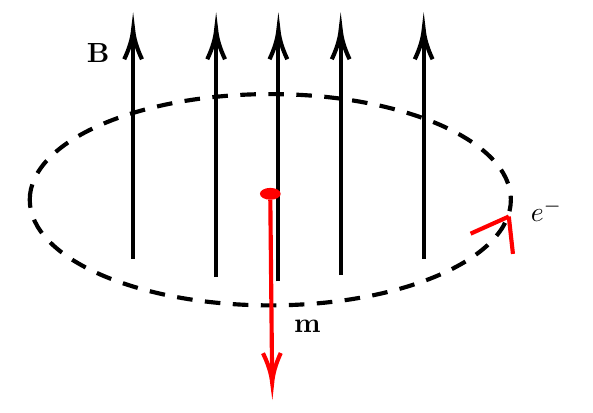
\begin{tikzpicture}[x=0.75pt,y=0.75pt,yscale=-1,xscale=1]
            %uncomment if require: \path (0,300); %set diagram left start at 0, and has height of 300

            %Shape: Ellipse [id:dp8639813058390806] 
            \draw  [dash pattern={on 5.63pt off 4.5pt}][line width=1.5]  (190,122.1) .. controls (190,93.99) and (241.89,71.2) .. (305.9,71.2) .. controls (369.91,71.2) and (421.8,93.99) .. (421.8,122.1) .. controls (421.8,150.21) and (369.91,173) .. (305.9,173) .. controls (241.89,173) and (190,150.21) .. (190,122.1) -- cycle ;
            %Straight Lines [id:da903094079444487] 
            \draw [line width=1.5]    (339.8,158.44) -- (339.8,43.2) ;
            \draw [shift={(339.8,40.2)}, rotate = 450] [color={rgb, 255:red, 0; green, 0; blue, 0 }  ][line width=1.5]    (14.21,-4.28) .. controls (9.04,-1.82) and (4.3,-0.39) .. (0,0) .. controls (4.3,0.39) and (9.04,1.82) .. (14.21,4.28)   ;
            %Straight Lines [id:da8758986216628213] 
            \draw [line width=1.5]    (279.8,159.44) -- (279.8,43.2) ;
            \draw [shift={(279.8,40.2)}, rotate = 450] [color={rgb, 255:red, 0; green, 0; blue, 0 }  ][line width=1.5]    (14.21,-4.28) .. controls (9.04,-1.82) and (4.3,-0.39) .. (0,0) .. controls (4.3,0.39) and (9.04,1.82) .. (14.21,4.28)   ;
            %Straight Lines [id:da2789297257171335] 
            \draw [line width=1.5]    (309.8,161.44) -- (309.8,43.2) ;
            \draw [shift={(309.8,40.2)}, rotate = 450] [color={rgb, 255:red, 0; green, 0; blue, 0 }  ][line width=1.5]    (14.21,-4.28) .. controls (9.04,-1.82) and (4.3,-0.39) .. (0,0) .. controls (4.3,0.39) and (9.04,1.82) .. (14.21,4.28)   ;
            %Straight Lines [id:da41807307836230745] 
            \draw [line width=1.5]    (239.8,150.44) -- (239.8,43.2) ;
            \draw [shift={(239.8,40.2)}, rotate = 450] [color={rgb, 255:red, 0; green, 0; blue, 0 }  ][line width=1.5]    (14.21,-4.28) .. controls (9.04,-1.82) and (4.3,-0.39) .. (0,0) .. controls (4.3,0.39) and (9.04,1.82) .. (14.21,4.28)   ;
            %Straight Lines [id:da9769541952675111] 
            \draw [line width=1.5]    (379.8,150.44) -- (379.8,43.2) ;
            \draw [shift={(379.8,40.2)}, rotate = 450] [color={rgb, 255:red, 0; green, 0; blue, 0 }  ][line width=1.5]    (14.21,-4.28) .. controls (9.04,-1.82) and (4.3,-0.39) .. (0,0) .. controls (4.3,0.39) and (9.04,1.82) .. (14.21,4.28)   ;
            %Straight Lines [id:da07955449336800569] 
            \draw [color={rgb, 255:red, 255; green, 0; blue, 0 }  ,draw opacity=1 ][line width=1.5]    (420.8,130.2) -- (402.4,138.44) ;
            %Straight Lines [id:da5605227952576148] 
            \draw [color={rgb, 255:red, 255; green, 0; blue, 0 }  ,draw opacity=1 ][line width=1.5]    (420.8,130.2) -- (422.8,148.2) ;
            %Straight Lines [id:da6729736350118587] 
            \draw [color={rgb, 255:red, 255; green, 0; blue, 0 }  ,draw opacity=1 ][line width=1.5]    (305.9,122.1) -- (306.77,207.2) ;
            \draw [shift={(306.8,210.2)}, rotate = 269.40999999999997] [color={rgb, 255:red, 255; green, 0; blue, 0 }  ,draw opacity=1 ][line width=1.5]    (14.21,-4.28) .. controls (9.04,-1.82) and (4.3,-0.39) .. (0,0) .. controls (4.3,0.39) and (9.04,1.82) .. (14.21,4.28)   ;
            %Shape: Ellipse [id:dp6844851006236772] 
            \draw  [draw opacity=0][fill={rgb, 255:red, 255; green, 0; blue, 0 }  ,fill opacity=1 ] (300.9,119.24) .. controls (300.9,120.82) and (303.14,122.1) .. (305.9,122.1) .. controls (308.66,122.1) and (310.9,120.82) .. (310.9,119.24) .. controls (310.9,117.66) and (308.66,116.39) .. (305.9,116.39) .. controls (303.14,116.39) and (300.9,117.66) .. (300.9,119.24) -- cycle ;

            % Text Node
            \draw (216,45.4) node [anchor=north west][inner sep=0.75pt]    {$\mathbf{B}$};
            % Text Node
            \draw (315.9,178.4) node [anchor=north west][inner sep=0.75pt]    {$\mathbf{m}$};
            % Text Node
            \draw (429.9,120.4) node [anchor=north west][inner sep=0.75pt]    {$e^{-}$};


        \end{tikzpicture}

    \end{center}

    Paramagnetism arises when the dipole moment\footnote{Fingers grip around direction of current (movement of \textbf{positive} charges, direction of thumb is the direction of dipole moment) - Right Hand Grip Rule} of the electron orbital align with the external magnetic field, while diamagnetism is a result of the change in the speed of electron due to the external magnetic field. The orbital contribution to paramagnetism is a lot smaller as it is much harder to tilt the orbital then to change its spin.

    The motion of the electron can be approximated as a steady current (because the orbital period is extremely short), then the magnetic dipole can be written as
    \begin{equation}
        \mathbf{m}=I\pi R^2 \hat{z}= \frac{-e}{T}\pi R^2 \hat{z} =\frac{-ev}{2\pi R}\pi R^2 \hat{z}=\frac{-evR}{2}\hat{z}
    \end{equation}
    where $R$ is the radius of the orbit (the negative sign accounts for the negative charge of the electron, as current is always a positive quantity)(v is defined as positive when it is anti clockwise).

    This shows that the electron orbital will always be subject to a torque ($\mathbf{m} \times \mathbf{B}$). However, it is hard to tilt the orbital. A more significant effect would be the change in speed of the electron due to the external $\mathbf{B}$ field.

    Assuming uniform circular motion, the initial speed ($v_0$) is given by
    \begin{equation}
        m \frac{v_0^2}{R}=\frac{1}{4\pi\epsilon_0}\frac{e^2}{R^2}
    \end{equation}

    Let's assume that the  $\mathbf{B}$ field is perpendicular to the orbit, the new speed of the electron would be given by
    \begin{equation}
        m \frac{v_1^2}{R^2}=\frac{1}{4\pi\epsilon_0}\frac{e^2}{R^2}+ev_1B
    \end{equation}
    \begin{equation}
        ev_1B=\frac{m}{R}(v_1^2-v_0^2)=\frac{m}{R}(v_1-v_0)(v_1+v_0)=\frac{m}{R}(\Delta v)(v_1+v_0)
    \end{equation}
    Assuming difference between $v_1$ and $v_0$ is small, making $\Delta v$ the subject
    \begin{equation}
        \Delta v = \frac{eRB}{2m}
    \end{equation}
    \begin{equation}
        \boxed{\therefore \Delta \mathbf{m}=\frac{-e^2 R^2}{4m} \mathbf{B}}
    \end{equation}
\end{mybox}

\section{Vector potential of a rotating, charged sphere}
\begin{mybox}{red}{Problem Statement}
    A spherical shell of radius $R$, carrying a uniform surface charge $\sigma$, is  set spinning at angular velocity $\omega$. Find the vector potential it produces at point $r$.
\end{mybox}
Firstly, we will have to recall the equation for vector potential from a surface current density
$$\mathbf{A(r)}=\frac{\mu_0}{4\pi}\int \frac{\mathbf{K}}{r} da$$
% Gradient Info
\begin{figure}[!h]
    \centering


    % Gradient Info

    \tikzset {_vc3u1ao19/.code = {\pgfsetadditionalshadetransform{ \pgftransformshift{\pgfpoint{0 bp } { 0 bp }  }  \pgftransformscale{1 }  }}}
    \pgfdeclareradialshading{_ugbcaoebz}{\pgfpoint{0bp}{0bp}}{rgb(0bp)=(1,1,1);
        rgb(0bp)=(1,1,1);
        rgb(25bp)=(0.75,0.75,0.75);
        rgb(400bp)=(0.75,0.75,0.75)}
    \tikzset{every picture/.style={line width=0.75pt}} %set default line width to 0.75pt        

    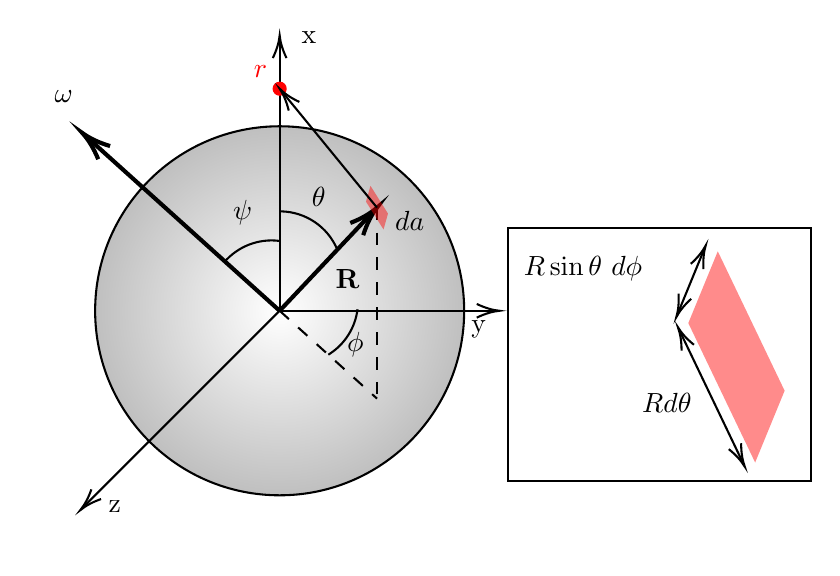
\begin{tikzpicture}[x=0.75pt,y=0.75pt,yscale=-1,xscale=1]
        %uncomment if require: \path (0,300); %set diagram left start at 0, and has height of 300

        %Shape: Circle [id:dp0650863396732182] 
        \path  [shading=_ugbcaoebz,_vc3u1ao19] (169,156.9) .. controls (169,107.8) and (208.8,68) .. (257.9,68) .. controls (307,68) and (346.8,107.8) .. (346.8,156.9) .. controls (346.8,206) and (307,245.8) .. (257.9,245.8) .. controls (208.8,245.8) and (169,206) .. (169,156.9) -- cycle ; % for fading 
        \draw   (169,156.9) .. controls (169,107.8) and (208.8,68) .. (257.9,68) .. controls (307,68) and (346.8,107.8) .. (346.8,156.9) .. controls (346.8,206) and (307,245.8) .. (257.9,245.8) .. controls (208.8,245.8) and (169,206) .. (169,156.9) -- cycle ; % for border 

        %Straight Lines [id:da35068944639340316] 
        \draw    (257.9,156.9) -- (257.9,26.2) ;
        \draw [shift={(257.9,24.2)}, rotate = 450] [color={rgb, 255:red, 0; green, 0; blue, 0 }  ][line width=0.75]    (10.93,-3.29) .. controls (6.95,-1.4) and (3.31,-0.3) .. (0,0) .. controls (3.31,0.3) and (6.95,1.4) .. (10.93,3.29)   ;
        %Straight Lines [id:da4826293228580578] 
        \draw    (257.9,156.9) -- (361.8,156.9) ;
        \draw [shift={(363.8,156.9)}, rotate = 180] [color={rgb, 255:red, 0; green, 0; blue, 0 }  ][line width=0.75]    (10.93,-3.29) .. controls (6.95,-1.4) and (3.31,-0.3) .. (0,0) .. controls (3.31,0.3) and (6.95,1.4) .. (10.93,3.29)   ;
        %Straight Lines [id:da6053235199019207] 
        \draw    (257.9,156.9) -- (163.21,251.59) ;
        \draw [shift={(161.8,253)}, rotate = 315] [color={rgb, 255:red, 0; green, 0; blue, 0 }  ][line width=0.75]    (10.93,-3.29) .. controls (6.95,-1.4) and (3.31,-0.3) .. (0,0) .. controls (3.31,0.3) and (6.95,1.4) .. (10.93,3.29)   ;
        %Straight Lines [id:da8404320731590209] 
        \draw [line width=1.5]    (257.9,156.9) -- (165.03,73.21) ;
        \draw [shift={(162.8,71.2)}, rotate = 402.02] [color={rgb, 255:red, 0; green, 0; blue, 0 }  ][line width=1.5]    (14.21,-4.28) .. controls (9.04,-1.82) and (4.3,-0.39) .. (0,0) .. controls (4.3,0.39) and (9.04,1.82) .. (14.21,4.28)   ;
        %Straight Lines [id:da917172748178974] 
        \draw [line width=1.5]    (257.9,156.9) -- (302.74,109.38) ;
        \draw [shift={(304.8,107.2)}, rotate = 493.34] [color={rgb, 255:red, 0; green, 0; blue, 0 }  ][line width=1.5]    (14.21,-4.28) .. controls (9.04,-1.82) and (4.3,-0.39) .. (0,0) .. controls (4.3,0.39) and (9.04,1.82) .. (14.21,4.28)   ;
        %Shape: Circle [id:dp9817752571413676] 
        \draw  [color={rgb, 255:red, 255; green, 0; blue, 0 }  ,draw opacity=1 ][fill={rgb, 255:red, 255; green, 0; blue, 0 }  ,fill opacity=1 ] (255,49.9) .. controls (255,48.3) and (256.3,47) .. (257.9,47) .. controls (259.5,47) and (260.8,48.3) .. (260.8,49.9) .. controls (260.8,51.5) and (259.5,52.8) .. (257.9,52.8) .. controls (256.3,52.8) and (255,51.5) .. (255,49.9) -- cycle ;
        %Straight Lines [id:da8152714675159394] 
        \draw [line width=0.75]  [dash pattern={on 4.5pt off 4.5pt}]  (257.9,156.9) -- (304.8,199.2) ;
        %Straight Lines [id:da3596356473594762] 
        \draw  [dash pattern={on 4.5pt off 4.5pt}]  (304.8,107.2) -- (304.8,199.2) ;
        %Shape: Parallelogram [id:dp020500604811702905] 
        \draw  [draw opacity=0][fill={rgb, 255:red, 255; green, 0; blue, 0 }  ,fill opacity=0.45 ] (299.5,104.33) -- (307.95,117.73) -- (310.1,110.07) -- (301.65,96.67) -- cycle ;
        %Shape: Arc [id:dp29063213769473806] 
        \draw  [draw opacity=0] (231.18,133.52) .. controls (237.64,125.96) and (247.63,121.93) .. (257.8,123.24) -- (254,153) -- cycle ; \draw   (231.18,133.52) .. controls (237.64,125.96) and (247.63,121.93) .. (257.8,123.24) ;
        %Straight Lines [id:da13766973298183638] 
        \draw [line width=0.75]    (304.8,107.2) -- (259.17,51.45) ;
        \draw [shift={(257.9,49.9)}, rotate = 410.7] [color={rgb, 255:red, 0; green, 0; blue, 0 }  ][line width=0.75]    (10.93,-3.29) .. controls (6.95,-1.4) and (3.31,-0.3) .. (0,0) .. controls (3.31,0.3) and (6.95,1.4) .. (10.93,3.29)   ;
        %Shape: Arc [id:dp748472790589076] 
        \draw  [draw opacity=0] (258.63,109) .. controls (270.14,109.25) and (280.97,116.14) .. (285.69,127.45) -- (258,139) -- cycle ; \draw   (258.63,109) .. controls (270.14,109.25) and (280.97,116.14) .. (285.69,127.45) ;
        %Shape: Arc [id:dp3545832365635029] 
        \draw  [draw opacity=0] (295.42,156.2) .. controls (294.35,164.74) and (289.63,172.77) .. (281.8,177.77) .. controls (281.65,177.86) and (281.5,177.96) .. (281.35,178.05) -- (265.65,152.49) -- cycle ; \draw   (295.42,156.2) .. controls (294.35,164.74) and (289.63,172.77) .. (281.8,177.77) .. controls (281.65,177.86) and (281.5,177.96) .. (281.35,178.05) ;
        %Shape: Rectangle [id:dp4634626491691636] 
        \draw  [fill={rgb, 255:red, 255; green, 255; blue, 255 }  ,fill opacity=0.75 ] (367.7,117.2) -- (513.8,117.2) -- (513.8,238.8) -- (367.7,238.8) -- cycle ;
        %Shape: Parallelogram [id:dp7933571242613435] 
        \draw  [draw opacity=0][fill={rgb, 255:red, 255; green, 0; blue, 0 }  ,fill opacity=0.45 ] (454.79,162.83) -- (486.99,230) -- (501.19,195.42) -- (468.99,128.25) -- cycle ;
        %Straight Lines [id:da9698449699127656] 
        \draw    (462.43,127.27) -- (449.75,158.15) ;
        \draw [shift={(448.99,160)}, rotate = 292.32] [color={rgb, 255:red, 0; green, 0; blue, 0 }  ][line width=0.75]    (10.93,-3.29) .. controls (6.95,-1.4) and (3.31,-0.3) .. (0,0) .. controls (3.31,0.3) and (6.95,1.4) .. (10.93,3.29)   ;
        \draw [shift={(463.19,125.42)}, rotate = 112.32] [color={rgb, 255:red, 0; green, 0; blue, 0 }  ][line width=0.75]    (10.93,-3.29) .. controls (6.95,-1.4) and (3.31,-0.3) .. (0,0) .. controls (3.31,0.3) and (6.95,1.4) .. (10.93,3.29)   ;
        %Straight Lines [id:da04109633277262925] 
        \draw    (450.66,166.63) -- (481.13,230.2) ;
        \draw [shift={(481.99,232)}, rotate = 244.39] [color={rgb, 255:red, 0; green, 0; blue, 0 }  ][line width=0.75]    (10.93,-3.29) .. controls (6.95,-1.4) and (3.31,-0.3) .. (0,0) .. controls (3.31,0.3) and (6.95,1.4) .. (10.93,3.29)   ;
        \draw [shift={(449.79,164.83)}, rotate = 64.39] [color={rgb, 255:red, 0; green, 0; blue, 0 }  ][line width=0.75]    (10.93,-3.29) .. controls (6.95,-1.4) and (3.31,-0.3) .. (0,0) .. controls (3.31,0.3) and (6.95,1.4) .. (10.93,3.29)   ;


        % Text Node
        \draw (267,21) node [anchor=north west][inner sep=0.75pt]   [align=left] {x};
        % Text Node
        \draw (348.8,159.9) node [anchor=north west][inner sep=0.75pt]   [align=left] {y};
        % Text Node
        \draw (174,247) node [anchor=north west][inner sep=0.75pt]   [align=left] {z\\};
        % Text Node
        \draw (137,48) node [anchor=north west][inner sep=0.75pt]   [align=left] {};
        % Text Node
        \draw (148,49.4) node [anchor=north west][inner sep=0.75pt]    {$\mathbf{\omega }$};
        % Text Node
        \draw (244,37.4) node [anchor=north west][inner sep=0.75pt]    {$\textcolor[rgb]{1,0,0}{r}$};
        % Text Node
        \draw (312.06,107.65) node [anchor=north west][inner sep=0.75pt]    {$da$};
        % Text Node
        \draw (234,102.4) node [anchor=north west][inner sep=0.75pt]    {$\psi $};
        % Text Node
        \draw (271.9,95.95) node [anchor=north west][inner sep=0.75pt]    {$\theta $};
        % Text Node
        \draw (288.9,165.95) node [anchor=north west][inner sep=0.75pt]    {$\phi $};
        % Text Node
        \draw (283.35,135.45) node [anchor=north west][inner sep=0.75pt]    {$\mathbf{R}$};
        % Text Node
        \draw (374.09,129.11) node [anchor=north west][inner sep=0.75pt]    {$R\sin \theta \ d\phi $};
        % Text Node
        \draw (431.09,195.11) node [anchor=north west][inner sep=0.75pt]    {$Rd\theta $};


    \end{tikzpicture}

\end{figure}
As shown in the figure above, we have to tilt our coordinate system by $\psi$ so as to make it easier to integrate. We can make our point of interest lie on the x axis, and the $\mathbf{\omega}$ vector lie on the x-z plane to make our lives easier. The first step to find surface current is to find the velocity of $da$.

Power of cross product: $\mathbf{v}=\mathbf{\omega}\times\mathbf{r}$ (not the other way round)
\footnote{
    $\begin{pmatrix}
            \hat{x} & \hat{y} & \hat{z} \\
            a_1     & a_2     & a_3     \\
            b_1     & b_2     & b_3
        \end{pmatrix}
        =(a_2b_3-a_3b_2)\hat{x}+(a_3b_1-a_1b_3)\hat{y}+(a_1b_2-a_2b_1)\hat{z}$}

$$\mathbf{v}=
    \begin{pmatrix}
        \hat{x}          & \hat{y}             & \hat{z}             \\
        \omega \cos \psi & 0                   & \omega \sin \psi    \\
        R\cos\theta      & R\sin\theta\cos\phi & R\sin\theta\sin\phi
    \end{pmatrix}$$

$$\mathbf{v}=-R\omega\sin\psi\sin\theta\cos\phi\hat{x}+(\omega\sin\psi R\cos\theta - \omega \cos \psi R \sin \theta \sin \phi)\hat{y}+\omega \cos \psi R \sin \theta\cos\phi \hat{z}$$
$$\mathbf{K}=\sigma \mathbf{v}$$




The integral would then be
$$\mathbf{A(r)}=\frac{\mu_0}{4\pi}\int_0^{2\pi} \int_0^\pi\frac{\mathbf{K}}{\sqrt{R^2+r^2-2Rr\cos\theta}} R^2 \sin\theta d\theta d\phi$$
Since the $\hat{x}$ and $\hat{z}$ components of $\mathbf{K}$ contain $\cos\phi$, after integration, those terms will vanish since
$$\int_0^{2\pi}\cos\phi d\phi =\int_0^{2\pi}\sin\phi d\phi=0 $$
Therefore,
$$\mathbf{A(r)}=\frac{\mu_0\sigma R^3 \omega \sin \psi}{2} \bigg(\int_0^\pi\frac{\mathbf{\sin\theta \cos\theta}}{\sqrt{R^2+r^2-2Rr\cos\theta}} d\theta \bigg) \hat{y}$$

After doing some crazy math and integration (which includes making the substitution: $u=\cos\theta$), we get

$$\mathbf{A(r)} =
    \begin{dcases*}
        \frac{\mu_0\sigma Rr \omega \sin \psi}{3}\hat{y}      & \text{inside the sphere}  \\
        \frac{\mu_0\sigma R^4 \omega \sin \psi}{3 r^2}\hat{y} & \text{outside the sphere}
    \end{dcases*}$$

To convert the solutions back to the orignal coordinate system, where the angular velocity vector coincides with the x axis, where our point of interest is located at $(r,\theta,\phi)$, we can do the conversion as such

\begin{figure}[!h]
    \centering



    % Gradient Info

    \tikzset {_p1ryku2p2/.code = {\pgfsetadditionalshadetransform{ \pgftransformshift{\pgfpoint{0 bp } { 0 bp }  }  \pgftransformscale{1 }  }}}
    \pgfdeclareradialshading{_7kobgnr4k}{\pgfpoint{0bp}{0bp}}{rgb(0bp)=(1,1,1);
        rgb(0bp)=(1,1,1);
        rgb(25bp)=(0.75,0.75,0.75);
        rgb(400bp)=(0.75,0.75,0.75)}
    \tikzset{every picture/.style={line width=0.75pt}} %set default line width to 0.75pt        

    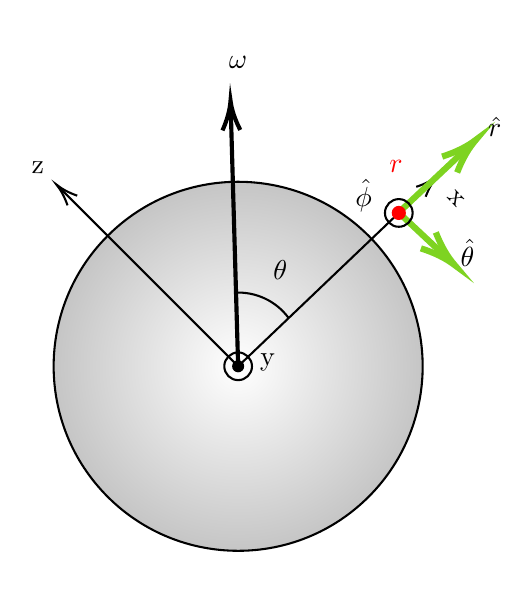
\begin{tikzpicture}[x=0.75pt,y=0.75pt,yscale=-1,xscale=1]
        %uncomment if require: \path (0,300); %set diagram left start at 0, and has height of 300

        %Shape: Circle [id:dp9079421007541035] 
        \path  [shading=_7kobgnr4k,_p1ryku2p2] (210.62,113.51) .. controls (246.13,79.61) and (302.4,80.91) .. (336.31,116.43) .. controls (370.21,151.94) and (368.9,208.22) .. (333.39,242.12) .. controls (297.88,276.02) and (241.6,274.71) .. (207.7,239.2) .. controls (173.8,203.69) and (175.1,147.41) .. (210.62,113.51) -- cycle ; % for fading 
        \draw   (210.62,113.51) .. controls (246.13,79.61) and (302.4,80.91) .. (336.31,116.43) .. controls (370.21,151.94) and (368.9,208.22) .. (333.39,242.12) .. controls (297.88,276.02) and (241.6,274.71) .. (207.7,239.2) .. controls (173.8,203.69) and (175.1,147.41) .. (210.62,113.51) -- cycle ; % for border 

        %Straight Lines [id:da09224944846459548] 
        \draw    (272,177.81) -- (366.54,87.57) ;
        \draw [shift={(367.99,86.18)}, rotate = 496.33] [color={rgb, 255:red, 0; green, 0; blue, 0 }  ][line width=0.75]    (10.93,-3.29) .. controls (6.95,-1.4) and (3.31,-0.3) .. (0,0) .. controls (3.31,0.3) and (6.95,1.4) .. (10.93,3.29)   ;
        %Straight Lines [id:da7596602693087713] 
        \draw    (272,177.81) -- (185.81,91.63) ;
        \draw [shift={(184.4,90.21)}, rotate = 405] [color={rgb, 255:red, 0; green, 0; blue, 0 }  ][line width=0.75]    (10.93,-3.29) .. controls (6.95,-1.4) and (3.31,-0.3) .. (0,0) .. controls (3.31,0.3) and (6.95,1.4) .. (10.93,3.29)   ;
        %Shape: Arc [id:dp2535563105704737] 
        \draw  [draw opacity=0] (270.46,142.34) .. controls (280.4,141.79) and (290.21,146.24) .. (296.28,154.5) -- (272.13,172.3) -- cycle ; \draw   (270.46,142.34) .. controls (280.4,141.79) and (290.21,146.24) .. (296.28,154.5) ;
        %Straight Lines [id:da7258560172888859] 
        \draw [color={rgb, 255:red, 126; green, 211; blue, 33 }  ,draw opacity=1 ][line width=2.25]    (349.34,103.75) -- (383.73,71.36) ;
        \draw [shift={(386.64,68.62)}, rotate = 496.72] [color={rgb, 255:red, 126; green, 211; blue, 33 }  ,draw opacity=1 ][line width=2.25]    (17.49,-5.26) .. controls (11.12,-2.23) and (5.29,-0.48) .. (0,0) .. controls (5.29,0.48) and (11.12,2.23) .. (17.49,5.26)   ;
        %Straight Lines [id:da1849979230355281] 
        \draw [line width=1.5]    (272,177.81) -- (268.41,52.85) ;
        \draw [shift={(268.33,49.85)}, rotate = 448.35] [color={rgb, 255:red, 0; green, 0; blue, 0 }  ][line width=1.5]    (14.21,-4.28) .. controls (9.04,-1.82) and (4.3,-0.39) .. (0,0) .. controls (4.3,0.39) and (9.04,1.82) .. (14.21,4.28)   ;
        %Straight Lines [id:da7755096466632982] 
        \draw [color={rgb, 255:red, 126; green, 211; blue, 33 }  ,draw opacity=1 ][line width=2.25]    (349.34,103.75) -- (373.48,126.38) ;
        \draw [shift={(376.4,129.12)}, rotate = 223.15] [color={rgb, 255:red, 126; green, 211; blue, 33 }  ,draw opacity=1 ][line width=2.25]    (17.49,-5.26) .. controls (11.12,-2.23) and (5.29,-0.48) .. (0,0) .. controls (5.29,0.48) and (11.12,2.23) .. (17.49,5.26)   ;
        %Shape: Circle [id:dp7600148976328078] 
        \draw  [color={rgb, 255:red, 255; green, 0; blue, 0 }  ,draw opacity=1 ][fill={rgb, 255:red, 255; green, 0; blue, 0 }  ,fill opacity=1 ] (347.4,101.83) .. controls (348.56,100.73) and (350.39,100.77) .. (351.5,101.93) .. controls (352.6,103.09) and (352.56,104.92) .. (351.4,106.03) .. controls (350.24,107.13) and (348.41,107.09) .. (347.3,105.93) .. controls (346.2,104.77) and (346.24,102.94) .. (347.4,101.83) -- cycle ;
        %Shape: Circle [id:dp6279405423900315] 
        \draw  [draw opacity=0][fill={rgb, 255:red, 0; green, 0; blue, 0 }  ,fill opacity=1 ] (270,175.72) .. controls (271.16,174.61) and (273,174.65) .. (274.1,175.81) .. controls (275.21,176.97) and (275.16,178.81) .. (274.01,179.91) .. controls (272.85,181.02) and (271.01,180.98) .. (269.91,179.82) .. controls (268.8,178.66) and (268.84,176.82) .. (270,175.72) -- cycle ;
        %Shape: Circle [id:dp5900036306516934] 
        \draw   (265.33,177.81) .. controls (265.33,174.13) and (268.32,171.14) .. (272,171.14) .. controls (275.69,171.14) and (278.67,174.13) .. (278.67,177.81) .. controls (278.67,181.5) and (275.69,184.48) .. (272,184.48) .. controls (268.32,184.48) and (265.33,181.5) .. (265.33,177.81) -- cycle ;
        %Shape: Circle [id:dp9424202248319924] 
        \draw   (342.73,103.93) .. controls (342.73,100.25) and (345.72,97.26) .. (349.4,97.26) .. controls (353.08,97.26) and (356.07,100.25) .. (356.07,103.93) .. controls (356.07,107.61) and (353.08,110.6) .. (349.4,110.6) .. controls (345.72,110.6) and (342.73,107.61) .. (342.73,103.93) -- cycle ;

        % Text Node
        \draw (376.59,90.56) node [anchor=north west][inner sep=0.75pt]  [rotate=-46.33] [align=left] {x};
        % Text Node
        \draw (171.1,77.51) node [anchor=north west][inner sep=0.75pt]  [rotate=-0.89] [align=left] {z\\};
        % Text Node
        \draw (267.29,15.17) node [anchor=north west][inner sep=0.75pt]  [rotate=-46.33] [align=left] {};
        % Text Node
        \draw (266.08,26.92) node [anchor=north west][inner sep=0.75pt]  [rotate=-359.02]  {$\boldsymbol{\omega }$};
        % Text Node
        \draw (343.32,77.37) node [anchor=north west][inner sep=0.75pt]  [rotate=-358.73]  {$\textcolor[rgb]{1,0,0}{r}$};
        % Text Node
        \draw (287.62,125.07) node [anchor=north west][inner sep=0.75pt]  [rotate=-1.58]  {$\theta $};
        % Text Node
        \draw (391,56.4) node [anchor=north west][inner sep=0.75pt]    {$\hat{r}$};
        % Text Node
        \draw (377.73,115.33) node [anchor=north west][inner sep=0.75pt]    {$\hat{\theta }$};
        % Text Node
        \draw (327,86.4) node [anchor=north west][inner sep=0.75pt]    {$\hat{\phi }$};
        % Text Node
        \draw (281.22,170.38) node [anchor=north west][inner sep=0.75pt]  [rotate=-1.28] [align=left] {y\\\\};


    \end{tikzpicture}



\end{figure}

Just use a bit of imagination (or refer to this diagram shown here). Also take note that $\boldsymbol{\omega}$ lie in the xz plane

Hence, we obtain the final solution in spherical coordinates
$$\mathbf{A(r)} =
    \begin{dcases*}
        \frac{\mu_0\sigma Rr \omega \sin \theta}{3}\boldsymbol{\hat{\phi}}      & \text{inside the sphere}  \\
        \frac{\mu_0\sigma R^4 \omega \sin \theta}{3 r^2}\boldsymbol{\hat{\phi}} & \text{outside the sphere}
    \end{dcases*}$$

To derive magnetic field from vector potential, we have to calculate it with $\mathbf{B}=\nabla \times \mathbf{A}$ (in spherical coordinates)

\begin{multline}
    \nabla \times \mathbf{A}=\frac{1}{r^2 \sin\theta}
    \begin{pmatrix}
        \hat{r}                     & r\hat{\boldsymbol{\theta}}      & r\sin\hat{\boldsymbol{\phi}}  \\
        \frac{\partial}{\partial r} & \frac{\partial}{\partial\theta} & \frac{\partial}{\partial\phi} \\
        A_r                         & rA_\theta                       & r\sin\theta A_\phi
    \end{pmatrix}
    =\frac{1}{r^2 \sin\theta}\begin{pmatrix}
        \hat{r}                     & r\hat{\theta}                   & r\sin\hat{\phi}               \\
        \frac{\partial}{\partial r} & \frac{\partial}{\partial\theta} & \frac{\partial}{\partial\phi} \\
        0                           & 0                               & r\sin\theta A_\phi
    \end{pmatrix}
    \\=\frac{1}{r^2 \sin\theta}\bigg(\frac{\partial}{\partial \theta} (r\sin\theta A_\phi)\hat{r}-\frac{\partial}{\partial r} (r\sin\theta A_\phi)r\hat{\boldsymbol{\theta}}\bigg)
\end{multline}

\begin{equation}
    \mathbf{B} =
    \begin{dcases*}
        \frac{2}{3}\mu_0 R \omega \sigma (\cos\theta \hat{r}-\sin \theta \hat{\boldsymbol{\theta}})      & \text{inside the sphere}  \\
        \frac{\mu_0 R^4 \omega \sigma}{3r^3} (2\cos\theta \hat{r}+\sin \theta \hat{\boldsymbol{\theta}}) & \text{outside the sphere}
    \end{dcases*}
\end{equation}

\section{Magnetisation}
The magnetisation, $\mathbf{M}$ is defined as the magnetic dipole moment per unit volume.
Since $\nabla \times \mathbf{M}=\mathbf{J_b}$, where $\mathbf{J_b}$ refers to the \textbf{bound current}. Bound current refers to \textit{invisible} current in the magnet due to magnetisation. There is another type of current called \textbf{free current} ($\mathbf{J_f}$). This is the current due to a battery, or a voltage source etc. In the case where both $\mathbf{J_f}$ and $\mathbf{J_b}$ are steady currents, we can apply the equation:
\begin{equation}
    \nabla \times \mathbf{B} = \mu_0 (\mathbf{J_f}+\mathbf{J_b})
\end{equation}
After replacing $\mathbf{J_b}$ with $\nabla \times \mathbf{M}$, and manipulation the equation, we get
\begin{equation}
    \nabla \times \bigg(\frac{\mathbf{B}}{\mu_0}-\mathbf{M}\bigg)=\mathbf{J_f}
\end{equation}
Now comes the cool part, we can replace $\big(\frac{\mathbf{B}}{\mu_0}-\mathbf{M}\big)$ with a quantity called $\mathbf{H}$, whose name is \textbf{Auxiliary Field}:
\begin{equation}
    \boxed{\nabla \times \mathbf{H}=\mathbf{J_f}}
    \quad\textsf{or}\quad
    \boxed{\oint \mathbf{H} \cdot d\mathbf{s} = I_\textsf{f,enc}}
\end{equation}

This equation is very elegant as it allows to express \textbf{Ampere's Law} in terms of free current alone, which is what we are able to control and measure.

Under certain circumstances however, we cannot use Ampere's Law methods to find $\mathbf{H}$ field. I asked this on stack exchange (\href{https://physics.stackexchange.com/questions/675083/when-can-we-use-amp%c3%a8res-law-methods-to-find-mathbfh-field}{my question})

\begin{mybox}{green}{When can we use Ampere's Law methods to find $\mathbf{H}$ field}
    Suppose that the H-field was composed of two parts. One of which had a curl of zero and the other which had a divergence of zero. Call them $\mathbf{H_{c=0}}$ and $\mathbf{H_{d=0}}$ respectively, such that

    $$\mathbf{H} = \mathbf{H_{c=0}} + \mathbf{H_{d=0}}\ .$$

    In which case Ampere's law
    $$\mathbf{J_f}=\nabla \times (\mathbf{H_{c=0}} + \mathbf{H_{d=0}})=\nabla \times \mathbf{H_{d=0}}$$

    The Helmholtz decomposition theorem tells us that any vector field can be represented by two such fields, so Amperes law will only tell us about the total H-field when it consists only of a divergence-free component. i.e. when $\mathbf{H}=\mathbf{H_{d=0}}$.

    In what circumstances is the H-field not entirely divergence free? When the magnetisation has a divergence.
    $$\mathbf{H}=\frac{\mathbf{B}}{\mu_0}-\mathbf{M}$$
    $$\nabla \cdot \mathbf{H_{c=0}} = - \nabla \cdot \mathbf{M}$$
\end{mybox}
In an infinitely long cylinder it is safe to assume the divergence of the magnetisation \footnote{ If the magnetisation is along the axis of the cylinder, then there is no magnetisation flux that enters or leaves the cylinder at the curved boundary. If the field varies along a coordinate perpendicular to the field direction then there is no divergence.}, and hence the H-field, is zero, and so the H-field only has a curl and is given by Ampere's law. (I always thought that divergence means gradient, but it is actually more like flux, see foonote).

A short cylinder has a divergence in magnetisation at the ends (and possibly also at parts of the curved boundary, if there is any component of the magnetisation unaligned with the cylinder), so the H-field has an additional curl-free term that isn't given by Ampere's law.

\section{Circuit}
\textit{2021 nodes connected to each other, find equivalent resistance between any 2 nodes.}
\begin{equation}
    \boxed{\textsf{Ans}=\frac{2R}{2021}}\nonumber
\end{equation}

\section{Things to remember}
Firstly, always remember that the following applies to discontinuity of E-field across a surface with charge density $\sigma$ (USAPhO 2008 A1):
\begin{equation}
    \Delta \mathbf{E}_\perp=\sigma/\epsilon_0
\end{equation}

\subsection{Grounding}
Grounding a conductor just means setting its voltage to $0$. One assumes the ground is an "infinite" reservoir of charge. Grounding a conductor means that now charge can flow in/out of the reservoir so that the final charge $Q$ on the conductor is such that its voltage is $0$. \textbf{This final value $Q$ is not necessarily $0$!}
